% !TeX spellcheck = en_US

\chapter{Design and Implementation}
\label{chap:ch4}
This chapter describes how the concept was implemented and presents the design of the plugin prototype.
First, a decision had to be made, for what \gls{IDE} the prototype would be implemented.
This decision as well as some reasoning for it can be found in \cref{sec:ch4:s1}.
Then the icons conceived in \cref{sec:ch3:s2} needed to be created, which is described in \cref{sec:ch4:s2}.
\Cref{sec:ch4:s3} presents the architecture for the prototype.
Finally, a few implementation details of the plugin, as well as some interesting parts of the implementation process, are described 
and the final prototype presented in \cref{sec:ch4:s4}.

\section{Choosing the IDE}
\label{sec:ch4:s1}
As the plugin prototype can only be implemented for one \gls{IDE} during the course of this thesis,
a decision had to be made, which \gls{IDE} to choose.
To support this decision the popularity, the support for creating plugins, and my prior experience were considered.

Based on these aspects the Eclipse \gls{IDE} \cite{burnette2005eclipse} was chosen.
It is one of the more popular \glspl{IDE} for Java \cite{geer2005eclipse}, 
which is one of the more widespread programming languages \cite{delorey2007programming}.
Additionally, Eclipse has extensive support for creating plugins \cite{clayberg2006eclipse}.
Finally, I already had some experiences with developing Eclipse plugins.

As the prototype plugin integrates the Gropius system into the eclipse \gls{IDE}, it has been named \gls{GropiusEI}.

\section{Icon Creation}
\label{sec:ch4:s2}
To create the icons described in \cref{sec:ch3:s2} the plan was made to combine multiple individual icons, one for each property, into many finished icons.
In the center of each icon is a symbol indicating the type of issue as this is the most relevant property.
The state of the issue is shown by the color of the main symbol because it is the least important property.
But to not discriminate people with partial or full colorblindness, a small black icon is also overlaid over the main icon.
The remaining three properties are visualized as annotations, small symbols displayed in the corners of the icon.
All of these parts are drawn as vector graphics so that the final icons can easily be scaled to any size.
One challenge while drawing is, that eclipse uses 16x16 pixel icons.
Therefore, all finished icons need to convey their information even if they are just 16x16 pixels.
This greatly reduces the possible detail in the parts.

\begin{figure}[!h]
	\centering
	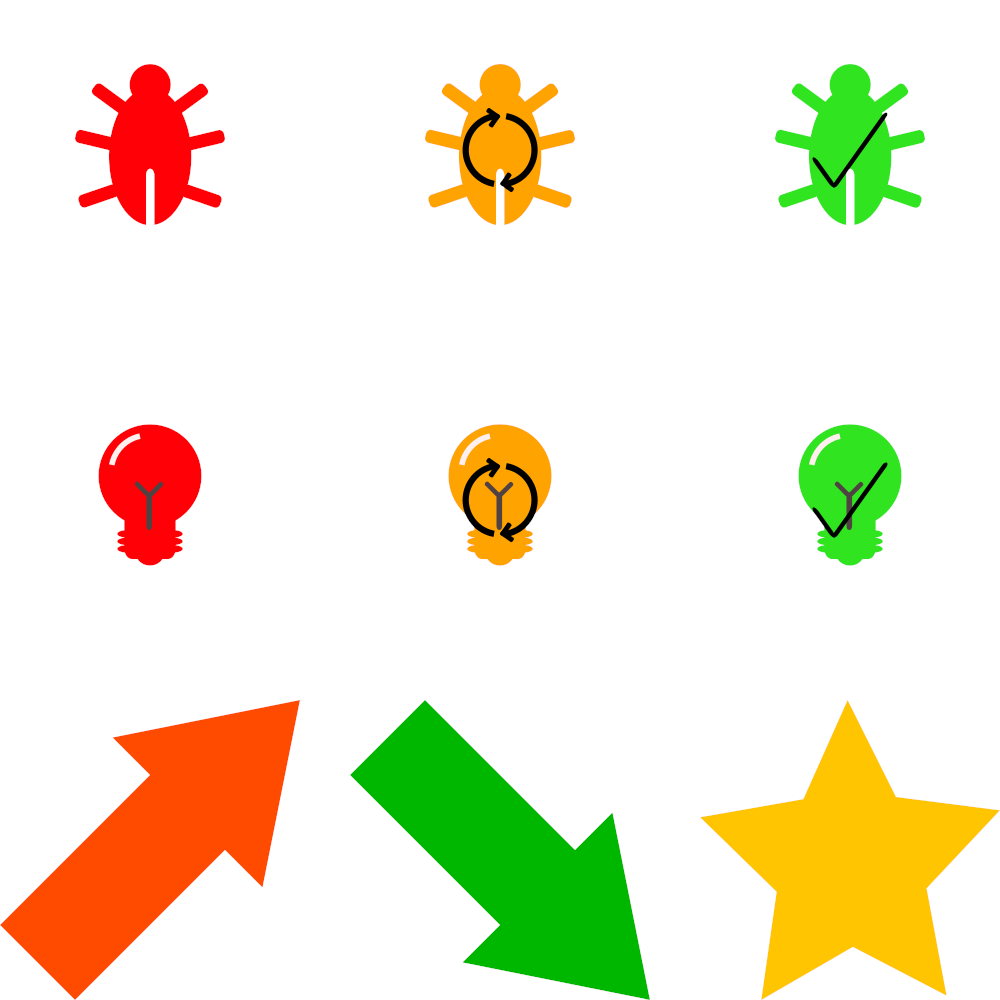
\includegraphics[width=0.5\textwidth]{graphics/iconParts.png}
	\caption{Issue Icon Parts}
	\label{fig:c4:icon_parts}
\end{figure}
\Cref{fig:c4:icon_parts} shows all the parts described above.
The first row contains the bugs from open to done, the second the enhancements, and the third the annotations for the other three properties.
The left-most annotation is included in the icon, when the issue causes problems in another project.
It is located on the top right of the finished icon.
The second symbol in the last row, is the annotation, for when the issue is just a symptom of an issue from another project.
On the final icons, this is shown on the top left.
The third symbol represents the fact, that the issue is assigned to the current developer and is added to the bottom left of the base icon.

\begin{figure}[!h]
	\centering
	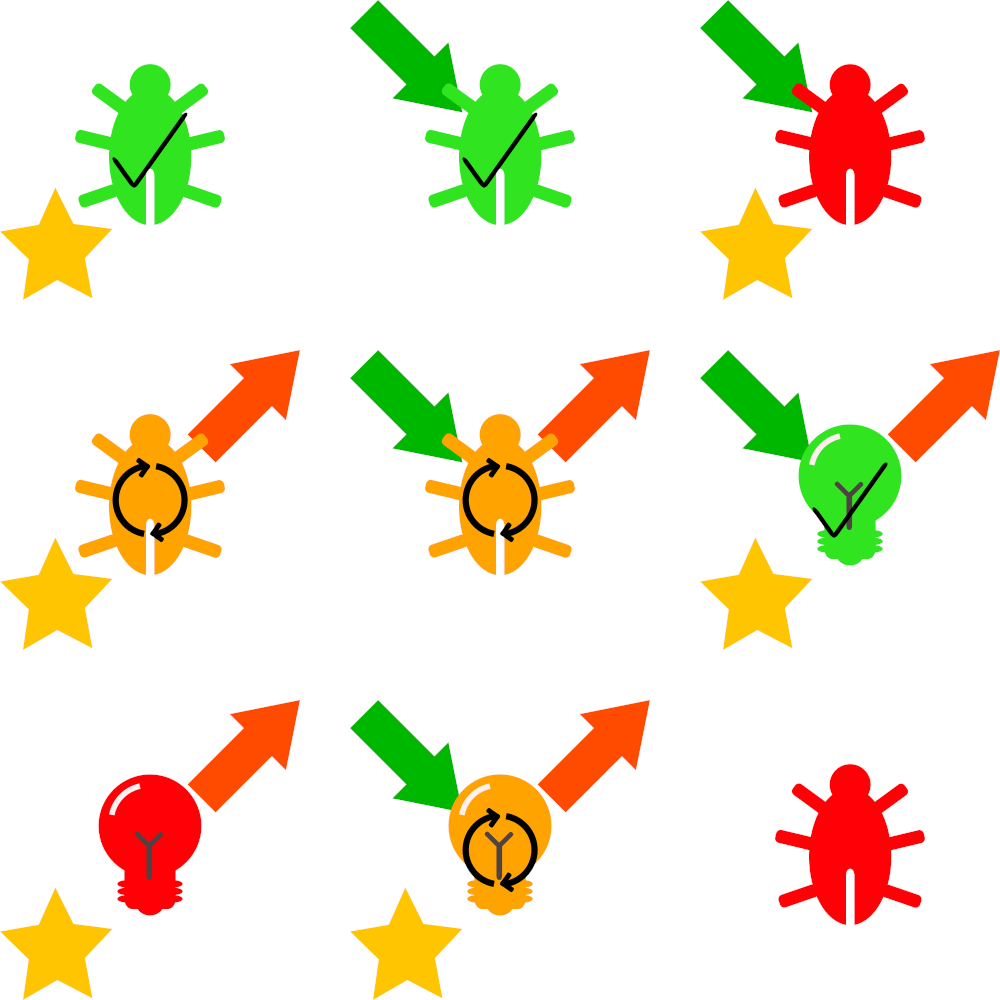
\includegraphics[width=0.5\textwidth]{graphics/iconCombinations.png}
	\caption{Issue Icon Examples}
	\label{fig:c4:icon_combinations}
\end{figure}
In \cref{fig:c4:icon_combinations} some examples of the final icons can be seen.
In total there are 48 different combinations of the above parts.
All of those need to be created and then converted into a pixel-based image format in multiple sizes, so they can be used.
This would be a very tedious manual task for one person.
Therefore, a small script was created, which does all that automatically and results in a folder with all combinations as \gls{PNG} files in the specified sizes.

\section{Plugin Architecture}
\label{sec:ch4:s3}
As described in \cref{sec:ch3:s3}, the plugin is split into several components for portability reasons.
Therefore, the prototype actually consists of a total of four eclipse plugins, as can be seen in \cref{fig:c4:component_diagram}.
Moreover, it was decided to use a model-driven software development approach similar to the one described in \cite{beydeda2005model}.
As a big part of the tool is a list and form for viewing and manipulating data, which can be described formally,
large parts of these two \gls{UI} elements can be automatically generated that way.

\begin{figure}[!h]
	\centering
	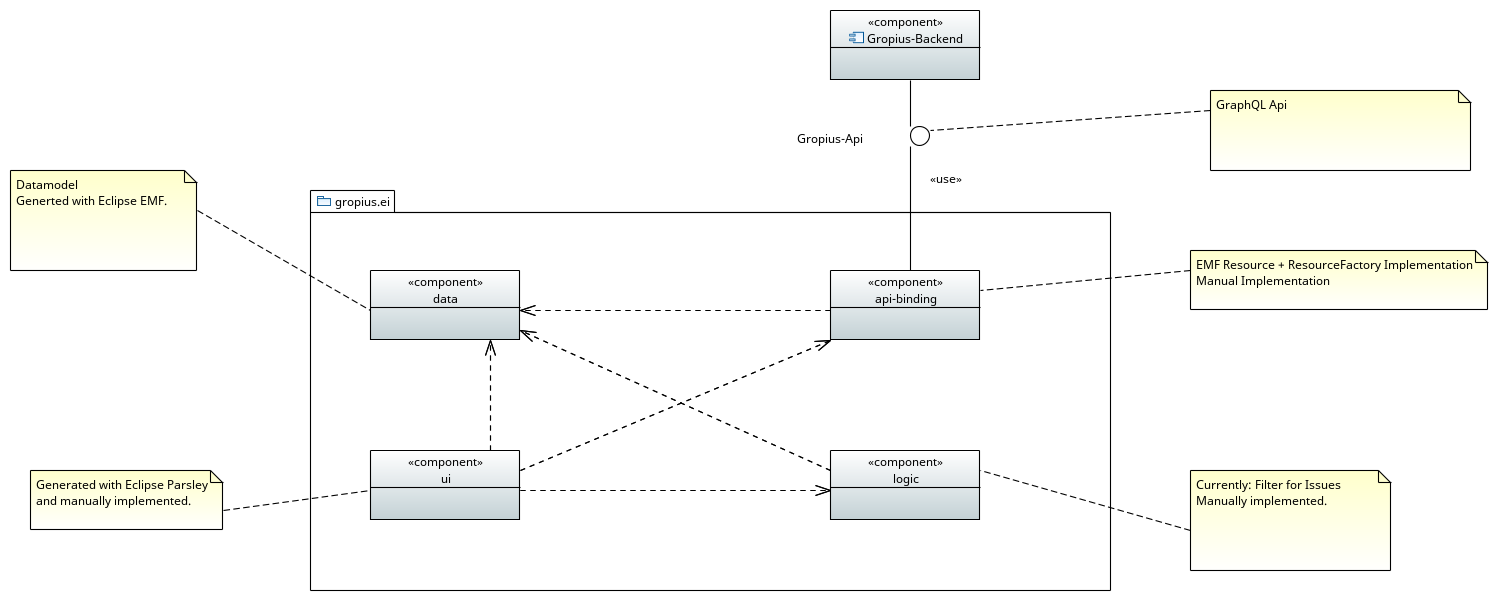
\includegraphics[width=\textwidth]{graphics/Component_Diagram.png}
	\caption{Prototype Component Diagram}
	\label{fig:c4:component_diagram}
\end{figure}

The plugin on the top left of \cref{fig:c4:component_diagram}, called \lstinline|data| contains the data model for the plugin. 
It is first modeled as an \gls{UML} model, then converted to an \gls{EMF} ecore model and then the model code is generated based on that.
Ecore is the metamodel to represent models in the \gls{EMF} world \cite{steinberg2008emf}.

The plugin \lstinline|api-binding| is responsible for all communication with the Gropius back-end through the Gropius \gls{API}.
Additionally, it converts between the data format defined in the \lstinline|data| plugin in the format used by the \gls{API}.
As mentioned in \cref{ssec:ch2:ss1.2}, the \gls{API} provided by the Gropius system uses \gls{graphql}.
Therefore, the client needs to specify exactly what data is required and create mutations for any changes to be sent to the server.
To be able to create these mutations, the difference between the old and the new version of the change needs to be recorded.
Both, the specification of the required data as well as the creation of mutations is also done by this component.

The third plugin, just called \lstinline|ui|, implements all the \gls{UI} elements.
It is the only plugin of the four that directly interacts with the eclipse \gls{IDE}.
This way, it is the only plugin, which needs major changes when the tool is ported to another \gls{IDE}, which supports Java-based plugins.
It uses the eclipse parsley framework introduced by \cite{bettini2014developing} to generate the issue list and issue details view 
based on the data model from the \lstinline|data| component.

The \lstinline|logic| plugin holds all classes containing logic needed by the \lstinline|ui|, which not eclipse specific.
One example would be the classes for filtering the issues based on some properties.
They are used by the filters for the issue list but do not require any \gls{IDE} specific functions.

A separate eclipse plugin for the messaging component would likely make sense.
But it was not modeled, as the idea of the messaging component was dropped from this thesis, for time constraint reasons.

\begin{figure}[!h]
	\centering
	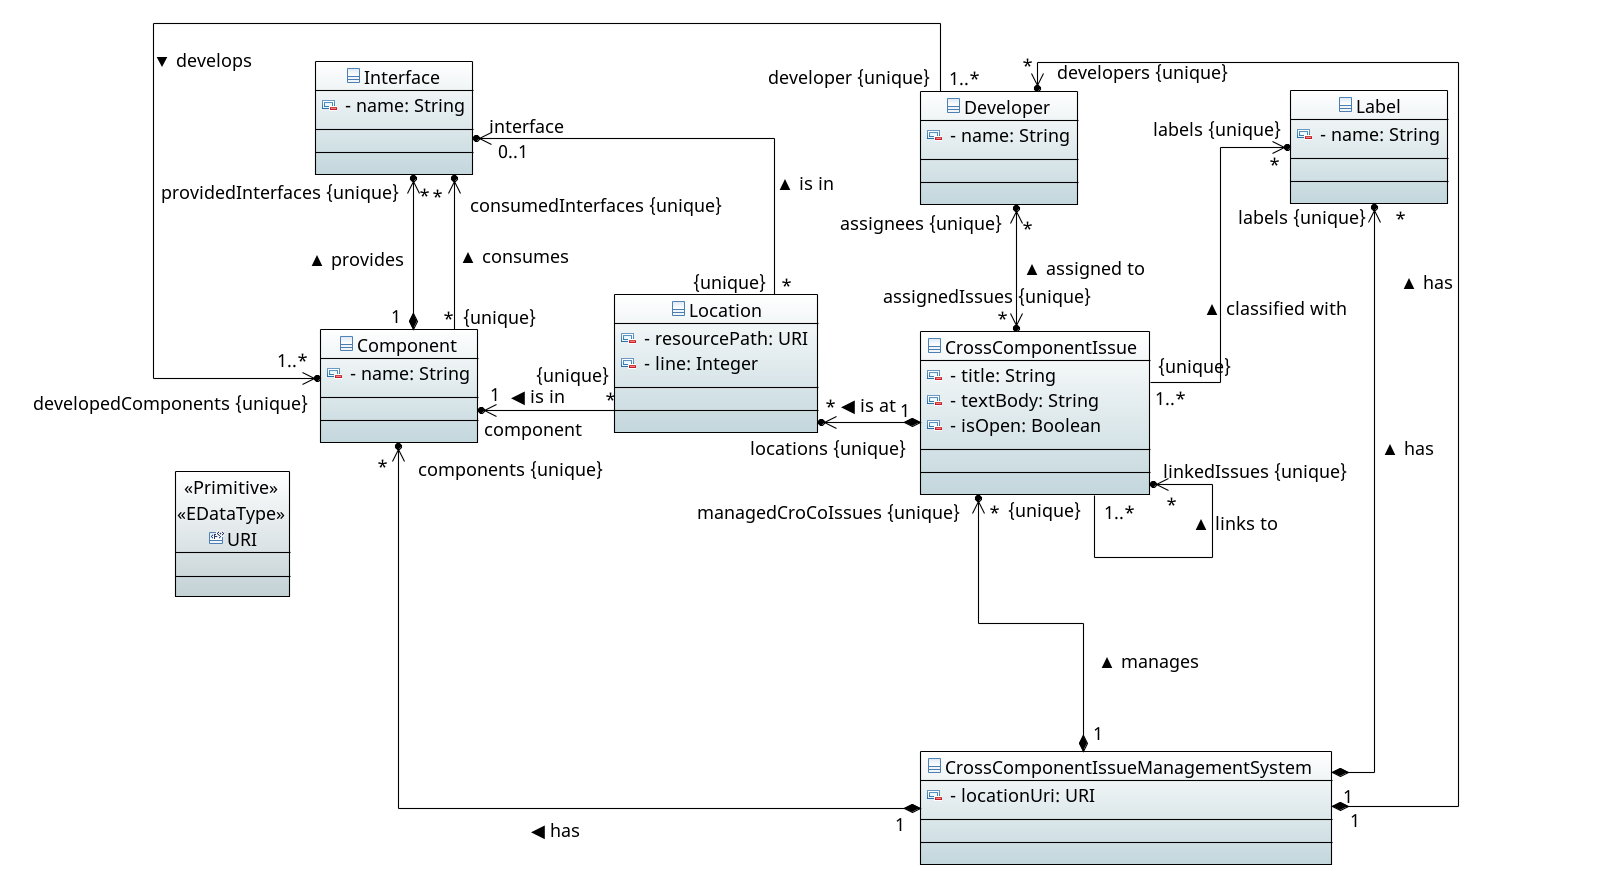
\includegraphics[width=\textwidth]{graphics/dataClassDiagram.png}
	\caption{Prototype Data Model Class Diagram}
	\label{fig:c4:data_class_diagram}
\end{figure}
The class diagram of the data model for \gls{GropiusEI} used to generate the \lstinline|data| component can be seen in \cref{fig:c4:data_class_diagram}.
At the core of the data model is the \lstinline|CrossComponentIssue|, with a title, text body, and a flag indicating whether it is open.
Additionally, it has various references to other objects, such as the assigned developers.

All \lstinline|CrossComponentIssue|s are contained within a \lstinline|CrossComponentIssueManagementSystem|.
That also has a list of all Labels, Developers, and Components relevant for the associated issues.
The tool always works with the issues contained in exactly one \lstinline|CrossComponentIssueManagementSystem|.

One important reference for the functionality of the tool is the \lstinline|linkedIssues| list of a \lstinline|CrossComponentIssue|.
It allows Gropius EI to show users linked issues as well as letting users navigate between them.

Another core concept of this model are the \lstinline|Location|s.
One issue can be at zero or more \lstinline|Location|s, which specify the resource and line the \lstinline|Location| is at.
Additionally, a \lstinline|Location| can be in a \lstinline|Component| or an \lstinline|Interface|.
\lstinline|Interface|s can be provided by exactly one \lstinline|Component| and consumed by any number of them.

\section{Plugin Implementation}
\label{sec:ch4:s4}
During the implementation phase, one of the biggest challenges was to understand and to correctly use eclipse parsley as well as \gls{EMF}.
Not a lot of documentation and tutorials could be found for either of them.
But as both of them are open source, answers for specific questions could be searched and found in the code itself.
However, this process is rather tedious and slow, so a lot of time was spent just looking through the source code of these frameworks.

Eclipse parsley is well suited for generating default \glspl{UI} for data models with basic support to customize them, 
but very little existing customization already available.
Therefore, a lot of the implementation work during this thesis was improving classes, which already exist in parsley 
and adding new variants of them, which allow further customization.
Most of them could be contributed to eclipse parsley after a little cleanup.

\begin{figure}[!h]
	\centering
	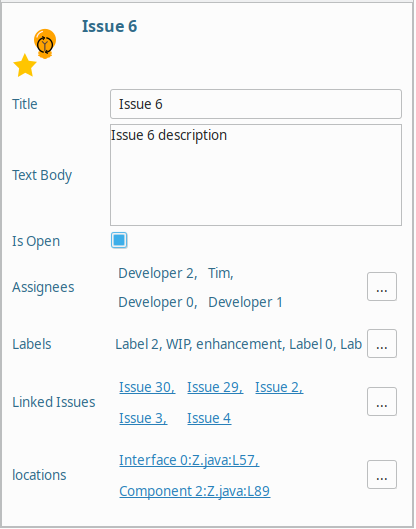
\includegraphics[width=0.5\textwidth]{graphics/screenshot_improvement_fromControl.png}
	\caption{Difference between original and new Control for lists}
	\label{fig:c4:screenshot_improvement_formControl}
\end{figure}
One example is the \gls{UI} element displayed inside a form for the value of properties, which are lists.
Parsley only supports to display the string representation of the complete list in one label.
The new implementation of the same class allows child classes to customize this by overwriting some methods.
Based on this some other classes were implemented using a grid of controls instead of a single Label.
This allows for nicer formatting when there are too many elements for one line.
Additionally, this allows the use of links as the control for each element, which is used for example by the \lstinline|linkedIssues| property.
The difference between the original and the improved version can be seen in \cref{fig:c4:screenshot_improvement_formControl}.
The control for the list \lstinline|Labels| is created by the original and you can see the last label is not completely readable.
The other controls are the new ones, with \lstinline|Developers| using a grid of labels and the other a grid of links.

Another significant amount of time was taken by working on the \lstinline|api-binding| plugin.
As the back-end was not ready in time, the component was implemented to work with a simple mock-up of the back-end.
Because of the fact, that the data from the \gls{API} is transformed into the data model generated with \gls{EMF}, 
the \gls{graphql} \gls{API} can not be used as intended.
Instead, all relevant data needs to be queried at once, every time the data is reloaded from the server.
This problem was detected too late to change the overall architecture of the plugin, 
mainly because the decision to switch to \gls{graphql} for the Gropius \gls{API} was made after the concept for \gls{GropiusEI} was already done.
However, to achieve this, a pretty complex query needs to be sent to the server.
Additionally, no appropriate java library could be found for using \gls{graphql} \glspl{API} without manually generating the queries and manually parsing the responses. 
In the end, some open-source ruby scripts \footnote{\url{https://github.com/Shopify/graphql_java_gen}} were used to generate helper classes from the Gropius \gls{graphql} schema.
The next problem was, that the mock-up of the back-end used to implement the \lstinline|api-binding| component is not sophisticated enough.
The returned data is not consistent in itself, which prevents a correct transformation into the \gls{GropiusEI} data model.
As the real back-end would not be ready in time, the decision was made to halt implementing the \lstinline|api-binding| plugin for now.
For the remainder of the thesis, the data is generated by a mock-data generator and stored in a file instead.

\subsection*{The Prototype}
Due to the lack of time, many of the features described in \cref{sec:ch3:s3} were never implemented.
Everything, that was implemented is presented in the next few paragraphs.

\begin{figure}[!h]
	\centering
	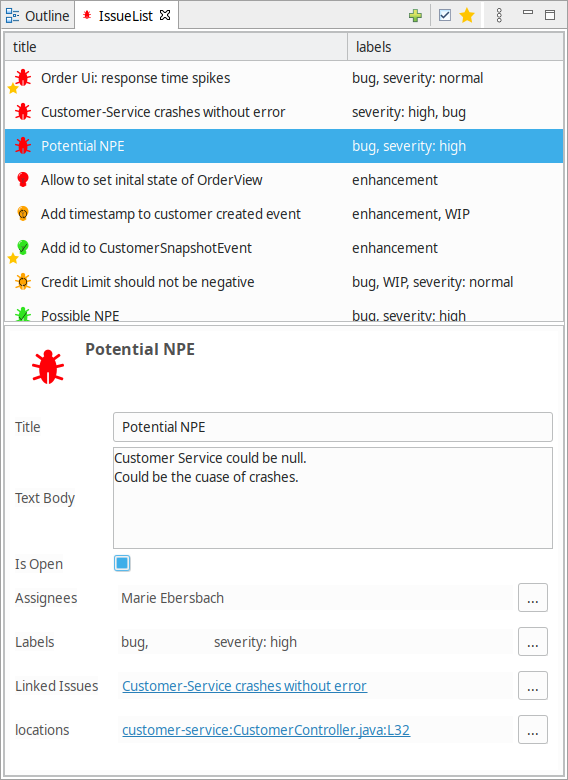
\includegraphics[width=0.4\textwidth]{graphics/screenshot_gropius_ei_issue_list.png}
	\caption{Prototype Issue List}
	\label{fig:c4:screenshot_issue_list}
\end{figure}
As stated in \cref{sec:ch3:s3} the main elements of \gls{GropiusEI} are the issue list and the issue detail view.
Deviating from the concept, those two elements are implemented in one big view element, as can be seen in \cref{fig:c4:screenshot_issue_list}.
This is the case because eclipse parsley provides such a view and implementing interactions between the two  parts is easier that way.

\begin{figure}[!h]
	\centering
	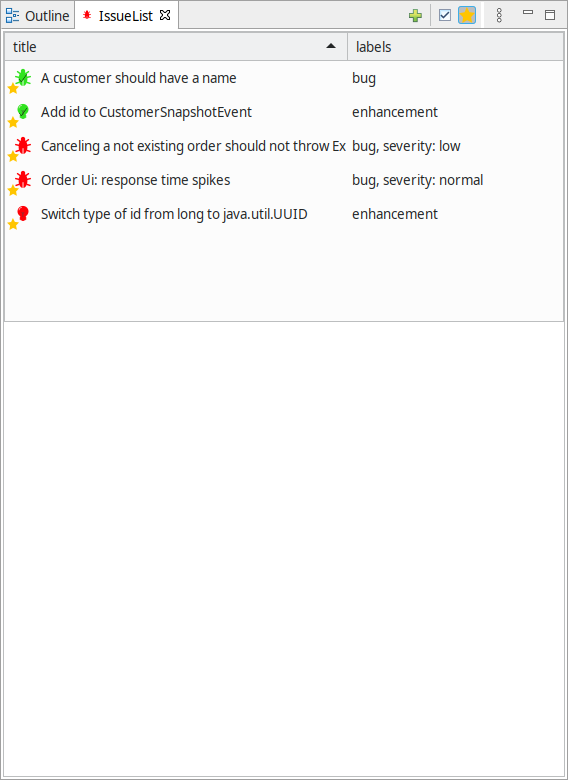
\includegraphics[width=0.4\textwidth]{graphics/screenshot_gropius_ei_issue_list_filtered_sorted.png}
	\caption{Prototype Issue List with Filter and Sorting}
	\label{fig:c4:screenshot_issue_list_filtered_sorted}
\end{figure}
As you can see in \cref{fig:c4:screenshot_issue_list_filtered_sorted}, the issue list also supports sorting by a column as well as filtering using the buttons in the bar on the top edge of the view.
Currently, only the filters \lstinline|Only show open issues| and \lstinline|Only show issues assigned to me| are implemented, 
but all the other filters specified in \cref{sec:ch3:s3} should be fairly straight forward to include.
Selecting the displayed columns is also possible through the menu on the top right.

\begin{figure}[!h]
	\centering
	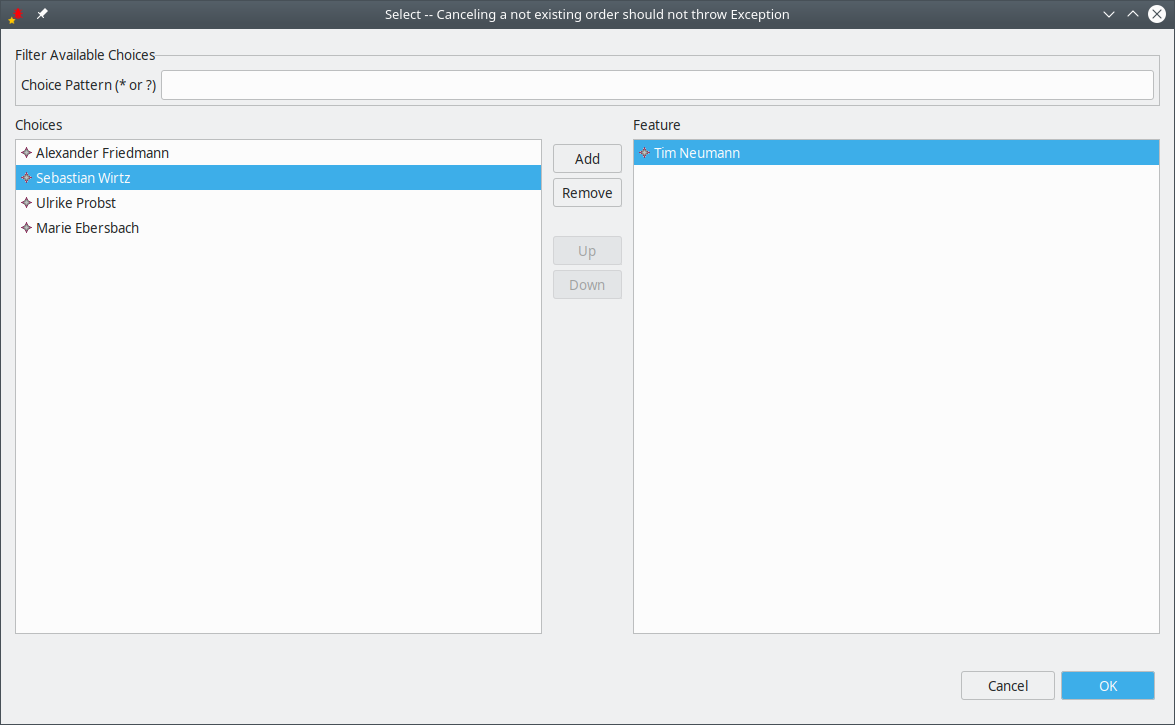
\includegraphics[width=0.7\textwidth]{graphics/screenshot_gropius_ei_edit_list.png}
	\caption{Prototype Edit Developers Dialog}
	\label{fig:c4:screenshot_edit_list}
\end{figure}

\begin{figure}[!h]
	\centering
	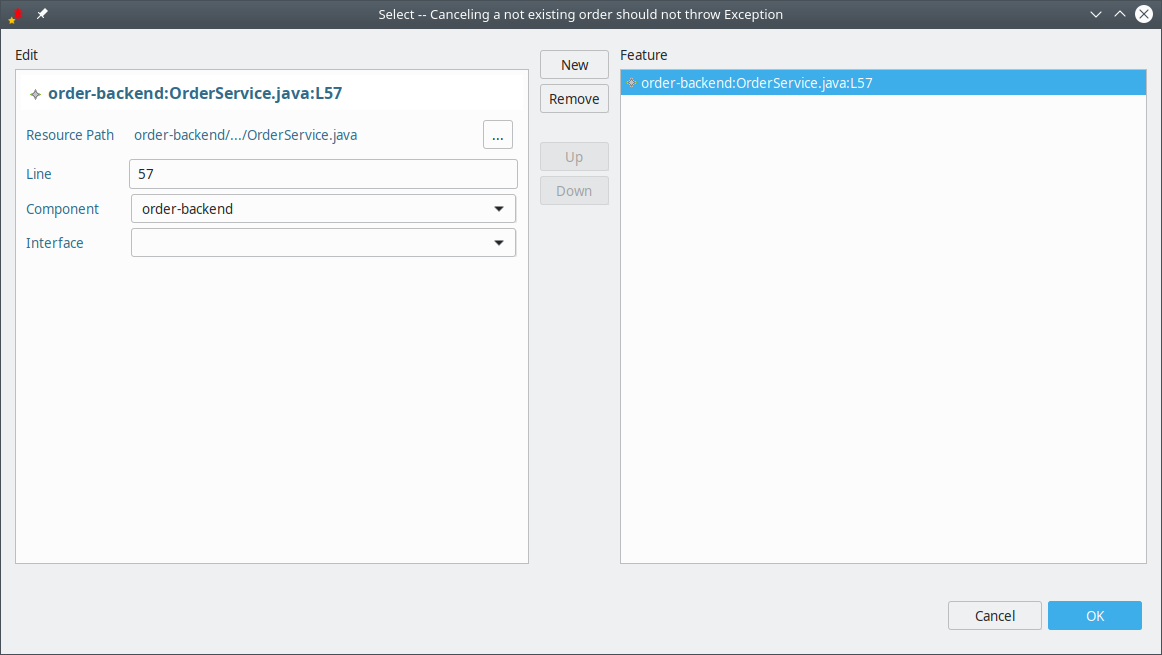
\includegraphics[width=0.7\textwidth]{graphics/screenshot_gropius_ei_edit_locations.png}
	\caption{Prototype Edit Locations Dialog}
	\label{fig:c4:screenshot_edit_locations}
\end{figure}

\Cref{fig:c4:screenshot_issue_list} also shows the details view, which is also a form for editing the selected issue.
The properties, which contain multiple values can be modified using the button to the right.
When that button is pressed a dialog similar to the one in \cref{fig:c4:screenshot_edit_list} is opened.
Changes done in the dialog are applied when the \lstinline|Ok| button is pressed.
The only exception is the \lstinline|locations| property.
For those a dialog (shown in \cref{fig:c4:screenshot_edit_locations}), which allows creating and editing locations is opened.
For the \lstinline|Linked Issues| and the \lstinline|Locations| each value is a link, 
selecting the correct issue in the list and jumping to that location in the code respectively.

The green plus button seen above the issue list in \cref{fig:c4:screenshot_issue_list} can be used to create new issues.
The feature for creating issues directly from some lines of code has not yet been implemented.
